\chapter{集成主动锁模激光器的构型}
\label{sec:related}

\fontsize{12bp}{14.4pt}

\section{谐振腔}
实验用样品为铒镱双掺。铒离子在$980nm$处的吸收截面较小,共同掺杂利用了镱离子在该波段处的大吸收截面,再通过振动将能量传递给周围的铒离子,以等效提升铒离子在该波段的泵浦吸收效率。\\
\begin{figure}[htbp]
    \centering
    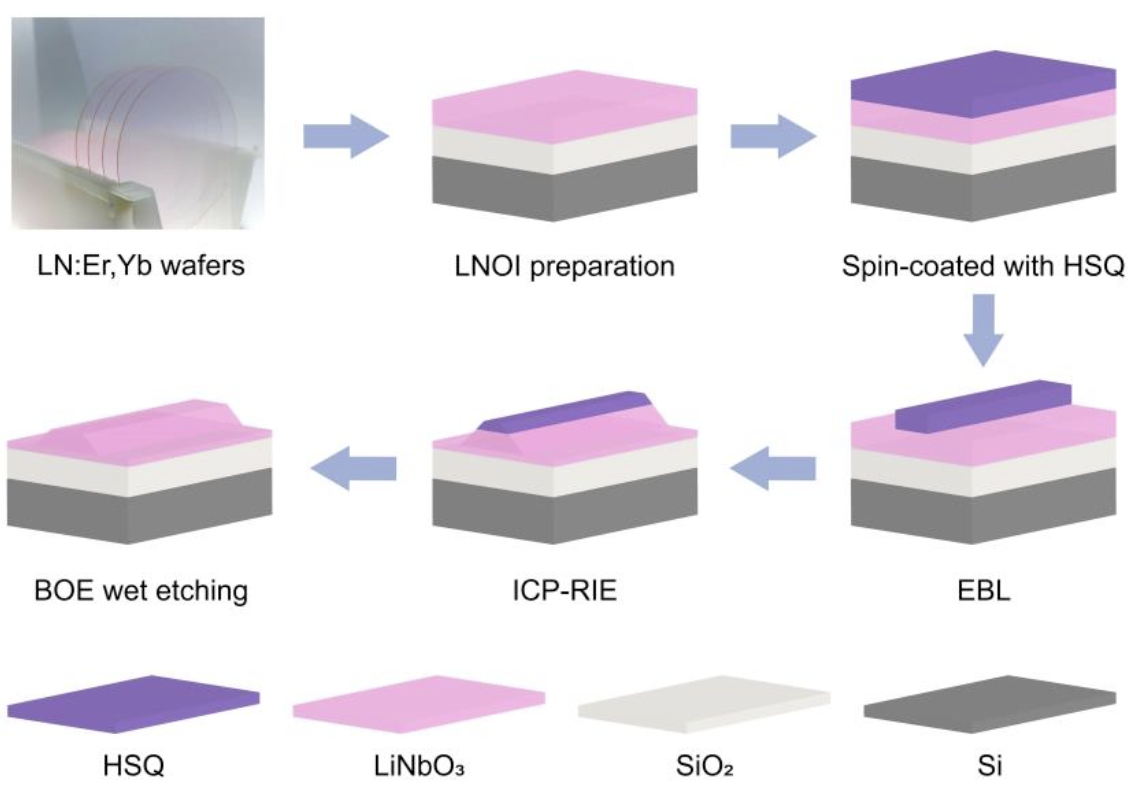
\includegraphics[width=0.7\linewidth]{figure/fig_1.png}
    \caption{铒镱双掺LNOI工艺流程}
    \label{fig:1}
\end{figure}
掺杂铌酸锂晶体通过Czochralski方法生长。再通过“smart-cut”技术制作LNOI晶圆。然后是半导体工艺:涂胶、曝光、蚀刻。
\begin{figure}[htbp]
    \centering
    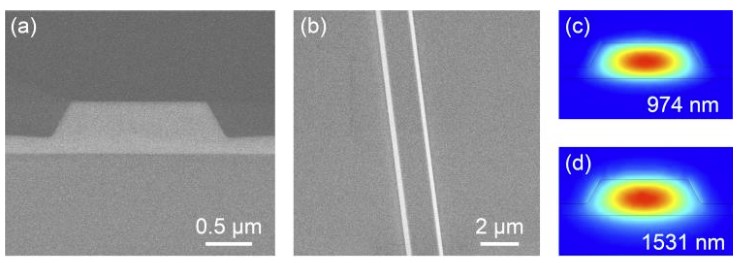
\includegraphics[width=0.7\linewidth]{figure/fig_7.png}
    \caption{a.SEM截面图。b.SEM俯视图。c,d. $974nm$和$1531nm$波长的模场分布。}
    \label{fig:enter-label}
\end{figure}
最终成品波导的厚度为$400nm$,底角为$60$度。
\begin{figure}[htbp]
    \centering
    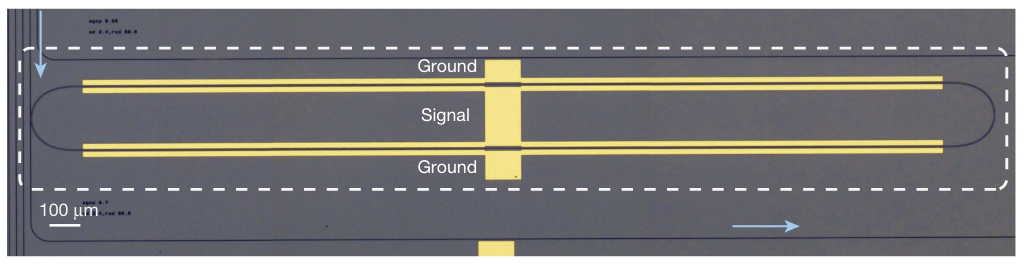
\includegraphics[width=0.95\linewidth]{figure/fig_8.png}
    \caption{波导与腔的构型图$~^{[2]}$}
    \label{fig:enter-label}
\end{figure}
为了利用最大的电光系数,腔被做成了跑道形,长边与z轴垂直。腔与外波导通过隐失波耦合。
\section{增益介质}
光信号的放大在光学中非常重要,常见的增益介质为稀土金属或III-IV族半导体。
掺铒光纤放大器在光纤通信中很成功,意味着铒离子也是集成平台上增益介质的极佳选择。$~^{[13]}$\\
使用Czochralski方法,在熔融阶段加入稀土元素,即可完成掺杂。\\
实际实验使用$1480nm$泵浦,因此仅需考虑铒离子的能级结构。$~^{[1]}$
\begin{figure}[htbp]
    \centering
    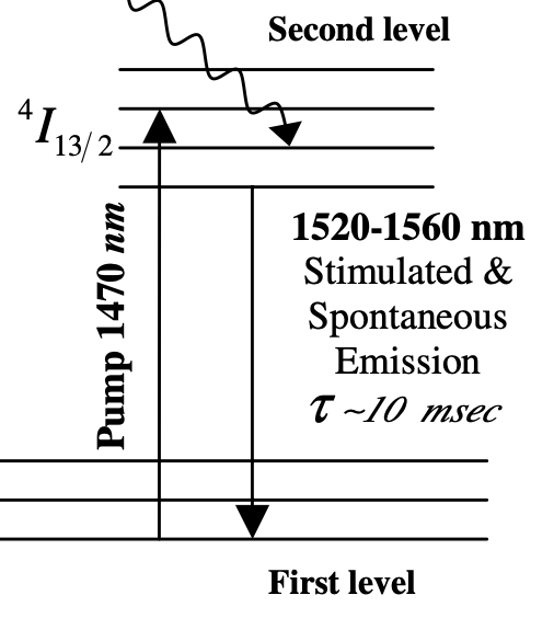
\includegraphics[width=0.5\linewidth]{figure/fig_27.png}
    \caption{铒离子的能级结构}
    \label{fig:enter-label}
\end{figure}
可用简化的三能级系统表示铒离子能级。下能级到上能级为泵浦。中间能级为一亚稳态,寿命约为$10ms$。上能级到中间能级的跃迁为无辐射跃迁,不释放或吸收光子,且速率较快。亚稳态到下能级的跃迁产生信号光。
\section{电光调制}
通过在平行于波导的两侧镀上金电极,可以在外部微波源的激励下产生面内垂直于波导方向的电场。可与TE模式光场产生最强的电光相互作用。\\
\begin{figure}[htbp]
    \centering
    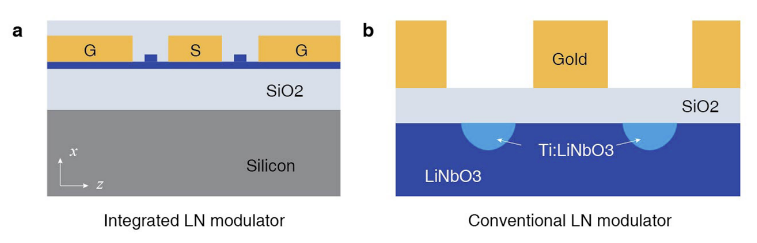
\includegraphics[width=0.8\linewidth]{figure/fig_10.png}
    \caption{带电极的波导截面图:a.强束缚波导,b.弱束缚波导}
    \label{fig:enter-label}
\end{figure}
G-S-G的电极构型充分利用了上下两段波导作为电光作用区域。通过交流探针,可将电信号施加到电极上。